\documentclass[../DoAn.tex]{subfiles}
\begin{document}

\section{Cơ sở lý thuyết}

\subsection{Mã hóa tích chập}

Mã hóa tích chập là một kỹ thuật mã hóa kênh quan trọng trong truyền thông số, được sử dụng rộng rãi trong các hệ thống như 4G/5G, vệ tinh, và truyền dẫn không dây. Khác với mã khối, mã tích chập xử lý dữ liệu thành một chuỗi liên tục, sử dụng các thanh ghi dịch và bộ cộng để tạo ra các bit mã hóa dựa trên cả bit hiện tại và các bit trước đó. Kỹ thuật này giúp phát hiện và sửa lỗi hiệu quả, đặc biệt trong môi trường nhiễu cao. Mã tích chập cân bằng giữa hiệu suất mã hóa và độ phức tạp tính toán, là nền tảng cho nhiều hệ thống truyền thông hiện đại \cite{noauthor_fundamentals_2015}. Các tham số chính quyết định hiệu năng mã hóa tích chập bao gồm:

\begin{itemize}

\item Chiều dài ràng buộc: số bit ảnh hưởng đến đầu ra mã hóa. Khi chiều dài ràng buộc tăng, khả năng sửa lỗi được cải thiện nhưng độ phức tạp giải mã tăng theo hàm mũ do số lượng trạng thái cần xử lý tăng.
\item Tốc độ mã: tỉ lệ bit thông tin/bit mã hóa. Tốc độ mã thấp cung cấp nhiều bit dư thừa giúp chống lỗi mạnh hơn trong kênh nhiễu, nhưng làm giảm thông lượng truyền dẫn. Kỹ thuật bỏ chọn bit dư có thể điều chỉnh linh hoạt tốc độ mã để cân bằng giữa độ tin cậy và hiệu suất.
\item Đa thức sinh: các kết nối giữa thanh ghi dịch và bộ cộng, thường biểu diễn bằng số hệ 8. Chúng quyết định khoảng cách tự do – tham số then chốt đánh giá khả năng phát hiện/sửa lỗi.

\end{itemize}

\subsection{Giải mã Viterbi} 

Thuật toán Viterbi là một phương pháp giải mã tối ưu cho mã hóa tích chập, được ứng dụng rộng rãi trong truyền thông số nhờ khả năng khôi phục dữ liệu chính xác ngay cả trong điều kiện nhiễu cao. Thuật toán hoạt động dựa trên nguyên lý quy hoạch động, duyệt qua tất cả các đường có thể trong lưới trạng thái để tìm ra chuỗi bit có khả năng cao nhất đã được phát đi. Nhờ hiệu quả và độ phức tạp vừa phải, Viterbi trở thành lựa chọn hàng đầu trong các hệ thống như 4G/5G, Wi-Fi, và thông tin vệ tinh. Thuật toán này kết hợp tính tối ưu và hiệu quả tính toán, đóng vai trò then chốt trong các hệ thống yêu cầu độ tin cậy cao \cite{a_viterbi_error_nodate}. Hiệu năng giải mã Viterbi phụ thuộc vào ba tham số chính:

\begin{itemize} 
\item Chiều dài ràng buộc: quyết định số trạng thái trong sơ đồ lưới. Khi chiều dài ràng buộc tăng, khả năng sửa lỗi được cải thiện do không gian tìm kiếm lớn hơn, nhưng độ phức tạp tính toán sẽ tăng theo hàm mũ.
\item Độ sâu truy ngược: xác định số bước để đưa ra quyết định giải mã cuối cùng. Độ sâu thường được chọn lớn hơn 5 lần chiều dài ràng buộc nhằm đảm bảo tỉ lệ lỗi bit dưới $10^{-5}$ trong kênh AWGN, nhưng tăng độ sâu truy ngược cũng dẫn đến tăng độ trễ xử lý và yêu cầu bộ nhớ lưu trữ đường đi lớn hơn.
\item Độ rộng lượng tử hóa: biểu thị số bit dùng để biểu diễn khoảng cách sai khác của đường đi. Giá trị 3-5 bit là tối ưu cho giải mã mềm, cân bằng giữa độ chính xác (cải thiện 2 dB SNR so với giải mã cứng) và tài nguyên phần cứng.
\end{itemize}

\section{Lựa chọn thiết kế}

Hiện nay, việc triển khai bộ mã hóa tích chập và giải mã Viterbi có thể được thực hiện bằng nhiều giải pháp khác nhau, mỗi phương pháp mang lại những ưu/nhược điểm riêng. CPU là lựa chọn linh hoạt và dễ triển khai nhờ thư viện phần mềm phong phú, nhưng độ trễ cao và kém hiệu quả khi xử lý song song khối lượng lớn dữ liệu \cite{noauthor_viterbi_nodate}. Trong khi đó, GPU cải thiện hiệu suất nhờ kiến trúc song song, nhưng tiêu thụ năng lượng lớn và đòi hỏi tối ưu hóa phức tạp \cite{liu_765-gbs_2025}. Giải pháp ASIC cho hiệu năng tối ưu và tiết kiệm điện năng, nhưng chi phí thiết kế đắt đỏ và không linh hoạt khi thuật toán thay đổi \cite{noauthor_tms320c6416_nodate}. FPGA cân bằng giữa hiệu suất và khả năng tùy biến, phù hợp cho các ứng dụng đòi hỏi độ trễ thấp, nhưng chưa tối ưu cho kiến trúc server truyền thống \cite{li_design_2012}. Cuối cùng, giải pháp SoC kết hợp CPU và FPGA khắc phục hạn chế của từng thành phần riêng lẻ bằng cách kết hợp xử lý phần mềm linh hoạt và tốc độ phần cứng, nhưng đòi hỏi thiết kế đồng bộ cả phần cứng lẫn phần mềm, dẫn đến độ phức tạp gia tăng \cite{mamarde_viterbi_2018}.

\begin{table}[H]
\centering{}
    \caption{So sánh các giải pháp triển khai thiết kế}
    \begin{tabular}{|p{0.13\linewidth} |p{0.35\linewidth}| p{0.35\linewidth}|}
        \hline
        \textbf{Giải pháp} & \textbf{Ưu điểm}  & \textbf{Nhược điểm}\\ \hline\hline
        CPU  & Linh hoạt, dễ triển khai  & Độ trễ cao, tốn tài nguyên khi xử lý song song   \\ \hline
        GPU  & Dễ tiếp cận, có khả năng xử lý song song  & Khó triển khai hơn CPU, tốn năng lượng   \\ \hline
        ASIC   & Hiệu năng cao, tiết kiệm năng lượng   & Chi phí thiết kế đắt, khó thay đổi thuật toán  \\ \hline
        FPGA        & Cân bằng hiệu năng và linh hoạt   & Chưa tối ưu cho kiến trúc server   \\ \hline
        SoC  & Xử lý song song, độ trễ thấp, mở rộng được   & Đòi hỏi thiết kế tối ưu phần cứng và phần mềm  \\ \hline
        \end{tabular}
    \label{table:So sánh các giải pháp triển khai thiết kế}
\end{table}

Nhìn chung, tùy vào yêu cầu cụ thể về hiệu suất, độ trễ, chi phí, và khả năng mở rộng mà ta có thể lựa chọn giải pháp phù hợp. Trong bối cảnh các hệ thống server hiện đại hướng đến kiến trúc lai, SoC hoặc FPGA tích hợp sẵn trong trung tâm dữ liệu đang nổi lên như xu hướng tối ưu cho bài toán mã hóa/giải mã quy mô lớn \cite{noauthor_acceleration_nodate}.

Để triển khai bộ mã hóa/giải mã dưới dạng server một cách hiệu quả, ta cần xây dựng yêu cầu chức năng và phi chức năng dựa vào những vấn đề cụ thể cần giải quyết:

\begin{table}[H]
\centering{}
    \caption{Yêu cầu chức năng và phi chức năng của hệ thống}
    \begin{tabular}{|p{0.25\linewidth} |p{0.28\linewidth} |p{0.37\linewidth}|}
        \hline
        \textbf{Vấn đề giải quyết} & \textbf{Yêu cầu chức năng}  & \textbf{Yêu cầu phi chức năng}\\ \hline\hline
        Tính ứng dụng  & Hỗ trợ tốc độ mã 1/2, 1/3, chiều dài ràng buộc 3-9 và tất cả các đa thức sinh  & Hệ thống phải cung cấp giao diện trực quan để người dùng dễ dàng thay đổi cấu hình\\ \hline
        Thông lượng xử lý  & Thuật toán giải mã được thiết kế theo kiến trúc Radix-4 \cite{black_140-mbs_1992}  & Hệ thống phải duy trì thông lượng xử lý ngay cả khi xử lý đồng thời nhiều luồng dữ liệu\\ \hline
        Khả năng tái cấu hình  & Có khả năng thay đổi cấu hình khi hệ thống đang hoạt động   & Việc thay đổi cấu hình phải không ảnh hưởng đến hoạt động liên tục\\ \hline
        Khả năng khử lỗi  & Độ sâu truy ngược lớn hơn 7 lần chiều dài ràng buộc \cite{a_viterbi_error_nodate}  & Tỷ lệ lỗi bit $<10^{-6}$ trong kênh AWGN \\ \hline
        Khả năng truy cập từ xa   &  Hệ thống hoạt động như một server  &  Luồng dữ liệu truyền tải phải được bảo mật\\ \hline
        Độ tin cậy  & Truyền tải dữ liệu qua giao thức TCP   & Có khả năng phục hồi nếu xảy ra lỗi mạng\\ \hline
        Độ linh hoạt  & Truyền dữ liệu dưới dạng các tập tin  & Các tập tin phải hoạt động độc lập với nhau\\ \hline
        \end{tabular}
\end{table}

Dựa trên các yêu cầu chức năng và phi chức năng, giải pháp SoC được lựa chọn làm nền tảng để thiết kế và triển khai bộ mã hóa tích chập và giải mã Viterbi. Do tính chất phức tạp đòi hỏi sự kết hợp giữa phần cứng và phần mềm, phương pháp Đồng thiết kế cứng mềm (Hardware/Software Codesign) trở thành lựa chọn tối ưu. Quy trình của phương pháp này bắt đầu từ việc xác định thông số kỹ thuật của hệ thống dựa trên các yêu cầu thiết kế. Sau đó, quá trình ước lượng chi phí được thực hiện để phân tích và tối ưu hóa tài nguyên trước khi tiến hành phân chia chức năng giữa phần cứng và phần mềm. Phần cứng tập trung vào các khối xử lý chuyên dụng nhằm đạt hiệu suất cao, trong khi phần mềm đảm nhận các tác vụ linh hoạt và điều khiển. Giai đoạn tiếp theo là đồng tổng hợp, nơi các đặc tả phần cứng và phần mềm được phát triển song song, bao gồm tổng hợp phần cứng và biên dịch phần mềm. Kết quả được kiểm chứng thông qua mô phỏng đồng bộ để đảm bảo tính chính xác và hiệu quả của hệ thống. Nếu kết quả chưa đạt yêu cầu, quy trình quay lại bước tinh chỉnh đặc tả để điều chỉnh thiết kế, tạo thành một vòng lặp khép kín cho đến khi đạt được kết quả tối ưu. Cách tiếp cận này đặc biệt phù hợp với các hệ thống phức tạp như bộ mã hóa tích chập và giải mã Viterbi, nơi đòi hỏi sự cân bằng giữa tốc độ xử lý phần cứng và tính mềm dẻo của phần mềm. Quy trình này được minh họa rõ ràng trong Hình \ref{fig:Phương pháp đồng thiết kế cứng mềm} \cite{gallery_hardwaresoftware_2003}.

\begin{figure}[H]
    \centering
    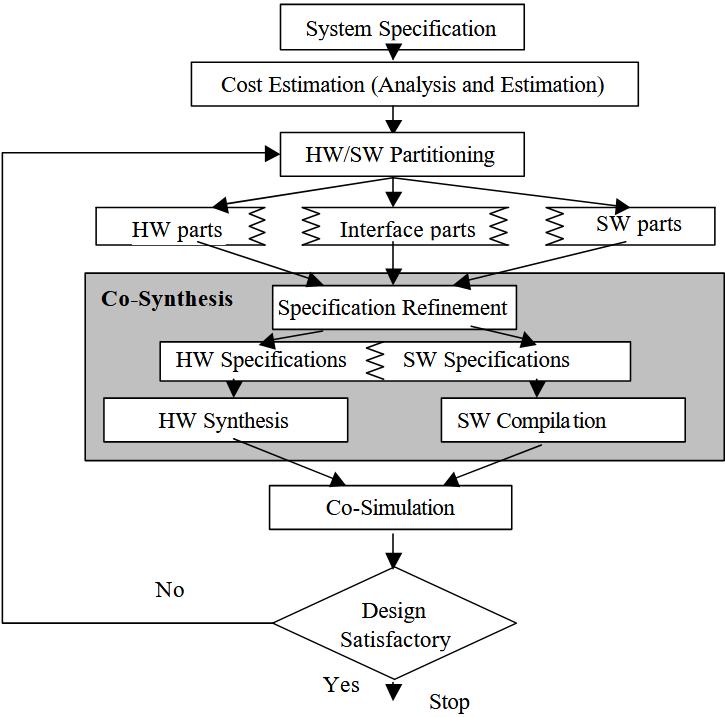
\includegraphics[width=\textwidth, height=0.33\textheight, keepaspectratio]{Hinhve/methodology.png}
    \caption{Quy trình trong phương pháp Đồng thiết kế cứng mềm}
    \label{fig:Phương pháp đồng thiết kế cứng mềm}
\end{figure}

\section{Công nghệ sử dụng}

\subsection{SoC}

Hệ thống trên chip (System-on-Chip - SoC) là một giải pháp tích hợp toàn bộ hệ thống máy tính vào một vi mạch duy nhất, bao gồm bộ xử lý, bộ nhớ, các khối xử lý tín hiệu số, và các giao diện ngoại vi. Trong đó, ZYNQ của Xilinx là một dòng SoC tiên tiến kết hợp lõi xử lý đa nhân với khả năng lập trình FPGA trên cùng một chip, mang lại sự linh hoạt và hiệu suất vượt trội. Kiến trúc ZYNQ chia thành hai phần chính: (i) phần xử lý (Processing System - PS) sử dụng lõi ARM Cortex, đảm nhiệm các tác vụ điều khiển phức tạp và giao tiếp với phần cứng bên ngoài; (ii) phần logic lập trình (Programmable Logic - PL) dựa trên công nghệ FPGA, cho phép thiết kế các khối xử lý tùy chỉnh để tăng tốc các thuật toán đòi hỏi tính toán song song như xử lý tín hiệu số, AI, hay mã hóa \cite{noauthor_amd_nodate}.

Liên kết giữa PS và PL trong ZYNQ được thực hiện thông qua các giao thức tốc độ cao như AXI, cho phép trao đổi dữ liệu hiệu quả giữa phần mềm chạy trên ARM và phần cứng tùy chỉnh trên FPGA. Nhờ đó, ZYNQ tối ưu hóa hiệu năng hệ thống bằng cách kết hợp sức mạnh xử lý tuần tự của CPU với khả năng xử lý song song và thời gian thực của FPGA \cite{noauthor_zynq-7000_2019}.

\subsection{AXI}
Giao thức AXI (Advanced eXtensible Interface) là một chuẩn giao tiếp quan trọng do ARM phát triển, được sử dụng rộng rãi trong các hệ thống SoC như Xilinx ZYNQ để kết nối hiệu quả giữa các khối xử lý (CPU, GPU), bộ nhớ và các module phần cứng tùy chỉnh trên FPGA. Trong đó, AXI-Stream là một biến thể không địa chỉ hóa của AXI, chuyên dụng cho các ứng dụng truyền dữ liệu tốc độ cao theo luồng liên tục, phù hợp với các tác vụ xử lý tín hiệu số hoặc truyền video. AXI cung cấp cơ chế truyền dữ liệu độc lập địa chỉ và dữ liệu, hỗ trợ burst transfers, và đảm bảo tính nhất quán trong hệ thống đa nhân \cite{noauthor_amba_nodate}.

\subsection{DMA}
DMA (Direct Memory Access) là cơ chế phần cứng cho phép các thiết bị ngoại vi truyền dữ liệu trực tiếp tới bộ nhớ hệ thống mà không cần sự can thiệp của CPU, giúp giảm tải xử lý và tăng hiệu suất hệ thống. Trong kiến trúc SoC như Xilinx ZYNQ, AXI DMA (AXI Direct Memory Access) là một module quan trọng, tận dụng giao thức AXI và AXI-Stream để kết nối hiệu quả giữa PS và PL. Với khả năng tối ưu hóa truyền dữ liệu giữa phần cứng và phần mềm, AXI DMA là thành phần không thể thiếu trong các thiết kế ZYNQ yêu cầu hiệu năng cao, từ IoT đến hệ thống nhúng phức tạp \cite{noauthor_introduction_nodate}.

\subsection{BRAM}
BRAM (Block RAM) là một dạng bộ nhớ được tích hợp sẵn trong kiến trúc PL của dòng Xilinx ZYNQ, đóng vai trò quan trọng trong việc lưu trữ và truy xuất dữ liệu tốc độ cao. Khác với bộ nhớ RAM cần truy cập qua bus hệ thống, BRAM nằm trực tiếp trên PL của ZYNQ, giúp giảm độ trễ và tăng hiệu suất cho các ứng dụng đòi hỏi thời gian phản hồi nhanh \cite{russell_what_2022}.

\subsection{ILA}
Integrated Logic Analyzer (ILA) là một công cụ debug mạnh mẽ được tích hợp trong Xilinx Vivado Design Suite, cho phép người dùng quan sát và phân tích tín hiệu bên trong thiết kế PL một cách trực tiếp. ILA hoạt động như một bộ phân tích logic cứng, sử dụng các tài nguyên logic và bộ nhớ khả dụng trên PL để thu thập và lưu trữ dữ liệu tín hiệu theo thời gian thực. Đặc biệt, ILA có mối quan hệ chặt chẽ với BRAM, BRAM thường được sử dụng làm bộ đệm lưu trữ dữ liệu tín hiệu thu thập bởi ILA, với khả năng lưu trữ lên đến hàng nghìn mẫu dữ liệu. Độ sâu cửa sổ debug của ILA phụ thuộc trực tiếp vào số lượng BRAM được cấp phát, trong khi tốc độ lấy mẫu được xác định bởi clock domain của tín hiệu cần debug. Khi thiết kế các hệ thống xử lý tín hiệu số phức tạp, việc tối ưu hóa việc sử dụng BRAM cho cả chức năng hệ thống lẫn nhu cầu debug bằng ILA trở thành một yếu tố quan trọng trong quá trình phát triển \cite{noauthor_integrated_nodate}.

\subsection{TCP}

TCP (Transmission Control Protocol) là một trong những giao thức cốt lõi của bộ giao thức TCP/IP, đóng vai trò quan trọng trong việc truyền dữ liệu đáng tin cậy và theo thứ tự giữa các thiết bị mạng. TCP cung cấp cơ chế kiểm soát lỗi, điều khiển luồng và đảm bảo dữ liệu được giao nhận chính xác giữa máy nguồn và máy đích. TCP là giao thức không thể thay thế cho các ứng dụng yêu cầu độ chính xác tuyệt đối \cite{noauthor_what_nodate}.

\subsection{lwIP}

lwIP (lightweight IP) là một thư viện mã nguồn mở, được thiết kế tối ưu cho các hệ thống nhúng có tài nguyên hạn chế (như vi điều khiển, FPGA, hoặc SoC). lwIP server là một triển khai của giao thức mạng dựa trên thư viện này, cho phép các thiết bị nhúng hoạt động như một máy chủ web, máy chủ TCP/UDP với bộ nhớ RAM chỉ từ vài chục KB và CPU tốc độ thấp \cite{noauthor_lwip_nodate}.

\subsection{Mesh Network}
Việc mở cổng mạng trên tường lửa router từ lâu đã là giải pháp phổ biến để truy cập thiết bị trong mạng nội bộ (LAN) từ bên ngoài Internet, nhưng nó đi kèm nhiều hạn chế: (i) quá trình cấu hình phức tạp, (ii) rủi ro bảo mật do mở cổng tường lửa, (iii) cần sự hỗ trợ từ nhà cung cấp mạng. Để khắc phục những vấn đề này, Mesh Network ra đời như một giải pháp hiện đại, cho phép các thiết bị kết nối trực tiếp với nhau qua Internet một cách an toàn và linh hoạt. \cite{mesh_network}.

Mesh Network là kiến trúc mạng phi tập trung, trong đó mỗi node (thiết bị) có thể giao tiếp trực tiếp với các node khác thông qua nhiều đường dẫn, tự động định tuyến lại nếu một liên kết bị lỗi. Một ví dụ điển hình của dịch vụ cung cấp Mesh Network là Tailscale, dịch vụ này xây dựng Mesh Network dựa trên giao thức WireGuard, giúp kết nối các thiết bị qua Internet như thể chúng cùng một mạng LAN mà không cần Port Forwarding hoặc cấu hình tường lửa phức tạp \cite{noauthor_tailscale_nodate}.


\end{document}